\section{Kriptologi: Kriptografi dan Kriptanalisis}

Banyak orang menganggap bahwa kriptografi hanyalah tentang membuat kode rahasia. Namun, dalam perspektif akademis, kriptografi adalah bagian dari bidang yang lebih luas yang disebut \textbf{Kriptologi}.

\subsection{Hubungan antara Kriptografi dan Kriptanalisis}

Kriptologi adalah studi ilmiah mengenai keamanan informasi yang terbagi menjadi dua cabang utama yang saling berlawanan namun saling melengkapi:

\begin{enumerate}
    \item \textbf{Kriptografi (\textit{Cryptography})}: Ilmu dan seni untuk membangun sistem penyandian yang aman. Fokus utamanya adalah menciptakan algoritma yang mampu menjaga kerahasiaan, integritas, dan otentikasi pesan.
    \item \textbf{Kriptanalisis (\textit{Cryptanalysis})}: Ilmu dan seni untuk memecahkan cipherteks menjadi plainteks tanpa mengetahui kunci yang digunakan. Fokus utamanya adalah mencari celah, kelemahan, atau pola dalam algoritma untuk membobol keamanan.
\end{enumerate}

Hubungan antara keduanya adalah sebuah siklus evolusi. Ketika seorang kriptografer menciptakan cipher baru yang dianggap aman, para kriptanalis akan mencoba memecahkannya. Jika berhasil, maka cipher tersebut dinyatakan tidak aman, dan kriptografer harus menciptakan metode baru yang lebih kuat. Itulah sebabnya kriptanalisis sering disebut sebagai "lawan" sekaligus "guru" bagi kriptografi.

\subsection{Sejarah Singkat Kriptanalisis}

Kriptanalisis sudah ada sejak abad ke-9, jauh sebelum komputer ditemukan. Salah satu tokoh paling berpengaruh adalah \textbf{Al-Kindi}, seorang ilmuwan Arab yang pertama kali memperkenalkan teknik \textbf{analisis frekuensi}. Ia menyadari bahwa dalam setiap bahasa, huruf-huruf tertentu muncul lebih sering daripada huruf lainnya. Dengan menghitung frekuensi kemunculan karakter dalam cipherteks, Al-Kindi dapat menebak huruf apa yang disandikan.

Sejarah mencatat bahwa keberhasilan kriptanalisis seringkali mengubah jalannya sejarah dunia. Contoh paling nyata adalah pemecahan kode \textit{Enigma} oleh pihak Sekutu pada Perang Dunia II, yang diperkirakan telah memperpendek durasi perang dan menyelamatkan jutaan nyawa.

\subsection{Kriptografi di Indonesia}

Di Indonesia, pengelolaan keamanan informasi dan sandi dikelola oleh lembaga negara yang kompeten, yaitu \textbf{Badan Siber dan Sandi Negara (BSSN)}. BSSN bertanggung jawab atas koordinasi keamanan siber dan kriptografi nasional. Selain itu, terdapat \textbf{Politeknik Siber dan Sandi Negara (PSSN)} sebagai lembaga pendidikan khusus yang mencetak tenaga ahli di bidang sandi dan keamanan siber.

Bagi mahasiswa yang tertarik mendalami sejarah kriptografi secara fisik, Indonesia memiliki \textbf{Museum Sandi} di Yogyakarta. Museum ini merupakan satu-satunya museum sandi di dunia yang menyimpan berbagai koleksi alat sandi bersejarah, mulai dari alat manual hingga mesin sandi mekanik yang pernah digunakan dalam perjuangan kemerdekaan dan pemerintahan Indonesia.

\begin{figure}[htbp]
  \centering
  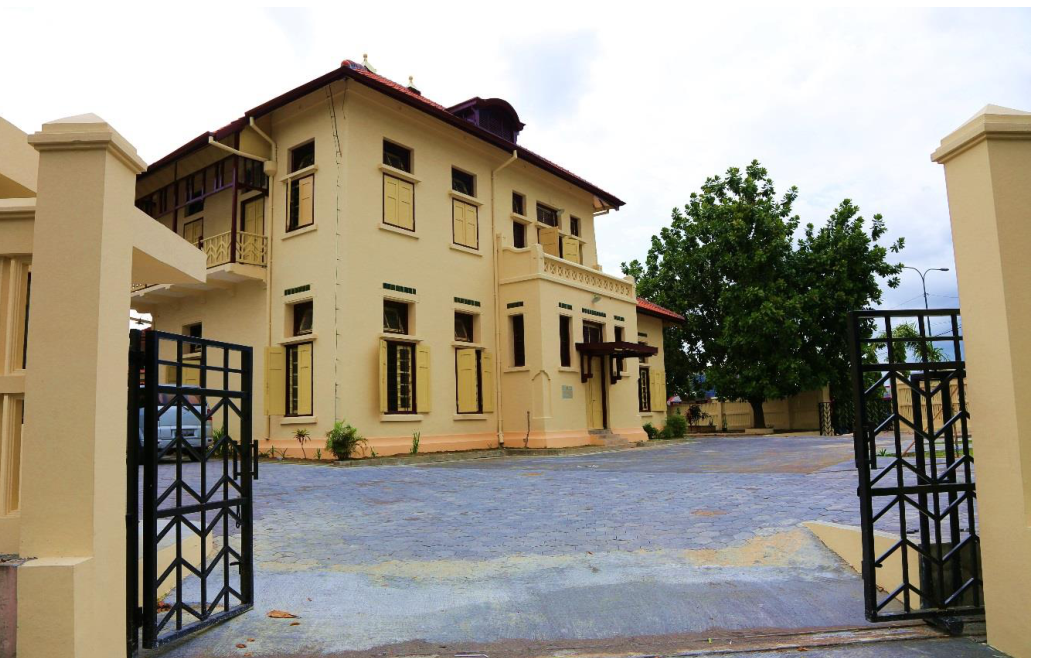
\includegraphics[width=0.6\textwidth]{referensi/01-Pengantar-Kriptografi-2026/images/llm/page_065_img_01.png}
  \caption{Museum Sandi Yogyakarta: Pusat pelestarian sejarah kriptografi di Indonesia.}
\end{figure}
